% Final project report for the Marie Curie team
% Written by William Harrington
% ECE478 Final Project
\documentclass[12pt]{article}
\usepackage{amsmath}
\usepackage{amssymb}
\usepackage{graphicx}
\usepackage{tabulary}
\usepackage{float}
\usepackage{hyperref}
\usepackage{tikz}
\usetikzlibrary{arrows, decorations.markings}

\tikzstyle{vecArrow} = [thick, decoration={markings,mark=at position
   1 with {\arrow[semithick]{open triangle 60}}},
   double distance=1.4pt, shorten >= 5.5pt,
   preaction = {decorate},
   postaction = {draw,line width=1.4pt, white,shorten >= 4.5pt}]
\tikzstyle{innerWhite} = [semithick, white,line width=1.4pt, shorten >= 4.5pt]

\begin{document}

\title{Final Project}%replace X with the appropriate number
\author{William Harrington, Sheetal Konnur\\ %replace with your name
ECE478} %if necessary, replace with your course title
\date{}
 
\maketitle
\small
\begin{description}
	\item[History and Introduction] \hfill \\ \\
		This report contains a detailed explanation of the Final project for the Marie Curie group. \\ \\
		The Marie Curie group was formed into the current state around Mid-November of 2015. Around this time Dr. Perkowski decided to move Will Harrington from the Einstein group to the Marie Curie group which only consisted of one member: Sheetal Konnur. The group was informed that they were to control the Marie Curie robot with a kinect in order to implement some sort of behavior.\\ \\
		Essentially, this is what is referred to as \textbf{Behavior-based robotics}. Behavior-based robotics is "..an approach in robotics that focuses on robots that are able to exhibit complex-appearing behaviors.." \footnote{https://en.wikipedia.org/wiki/Behavior-based\_robotics}. Upon learning this, the group embarked on using a kinect for controlling Marie Curie by using a raspberry pi 2 for image processing and an arduino with a poll driver to control the servos of the robot. However, after working on this for a few weeks, the team was informed by Dr. Perkowski that this is not what he wanted. Apparently, Marie Curie had a long storied past that the team was unaware of. Other students who had worked on Marie Curie already had done "better algorithms" for image processing and controlling the robot. What Dr. Perkowski wanted was for our group to evolve this work further. \\ \\
		At this point in the term, it was a long shot that a group of two students would be able to do what Dr. Perkowski wanted. The group decided to simply undertake a more refined version of homework 1. Homework 1 involved using a powerpoint to do scenario prototyping. Therefore, the kinect would be used to control the powerpoint and another means of controlling the robot would have to be triggered with the powerpoint. A Finite State Machine with probabilistic logic is also needed for this. \\ \\
		In conclusion, the final project for the Marie Curie group became a behavior-based robotics application with a focus on scenario prototyping using a finite state machine. \\ \\
	\item[Goals] \hfill \\
		\begin{enumerate}
			\item Use powerpoint for scenario prototyping
			\item Use kinect to control mouse on computer so that it can be used to click buttons within the powerpoint
			\item Use an arduino to drive the servo controller (Pololu)
			\item Trigger arduino using the firmata protocol
			\item Implement Finite State Machine with probabilistic logic for robot behavior
		\end{enumerate}
	\item[High level system model] \hfill \\
		\\
		\tikzstyle{int}=[draw, fill=blue!20, minimum size=2em]
		\tikzstyle{init} = [pin edge={to-,thin,black}]
		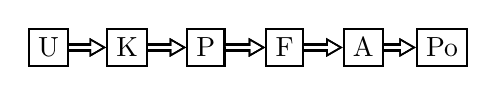
\begin{tikzpicture}[thick]
  			\node[draw,rectangle] (a) {U};
	  		\node[draw,rectangle,right of=a] (b) {K};
  			\node[draw,rectangle,right of=b] (c) {P};
  			\node[draw,rectangle,right of=c] (d) {F};
			\node[draw,rectangle,right of=d] (e) {A};
			\node[draw,rectangle,right of=e] (f) {Po};
			
  			% 1st pass: draw arrows
  			\draw[vecArrow] (a) to (b);
  			\draw[vecArrow] (b) to (c);
			\draw[vecArrow] (c) to (d);
			\draw[vecArrow] (d) to (e);
			\draw[vecArrow] (e) to (f);

  			% 2nd pass: copy all from 1st pass, and replace vecArrow with innerWhite
  			\draw[vecArrow] (a) to (b);
 		 	\draw[vecArrow] (b) to (c);
			\draw[vecArrow] (c) to (d);
			\draw[vecArrow] (d) to (e);
			\draw[vecArrow] (e) to (f);

  		% Note: If you have no branches, the 2nd pass is not needed
		\end{tikzpicture}
		\begin{itemize}
			\item U = User
			\item K = Kinect
			\item P = PowerPoint
			\item F = Firmata
			\item A = Arduino
			\item Po = Pololu
		\end{itemize}
		\textbf{High level system explanation} \\
		The high level system diagram shown above depicts the flow of inputs for our system. The user controls the mouse on the computer by using their hands while in front of a kinect. The kinect receives the input from the user and makes the appropriate mouse clicks on the computer. When the user clicks a button on the powerpoint, a program that uses the firmata protocol sends a signal to the arduino. The arduino then triggers the pololu controller to move the servos according to what behavior we want our robot to enact. 
		\newpage
	\item[Implementation] \hfill \\
		
		\textbf{Materials used}
		\begin{itemize}
			\item Windows Laptop
			\item Microsoft Kinect
			\item Arduino Uno
			\item Micro Maestro 6-Channel USB Servo Controller
		\end{itemize}
		
		\textbf{Required software}
		\begin{itemize}
			\item Microsoft PowerPoint
			\item Kinect Mouse \footnote{http://futuretechblog.com/?p=26}
			\item Python
			\begin{itemize}
				\item pyFirmata \footnote{https://pypi.python.org/pypi/pyFirmata/0.9.5} \footnote{https://github.com/tino/pyFirmata}
			\end{itemize}
			\item Arduino
			\begin{itemize}
				\item Firmata for Arduino \footnote{http://www.instructables.com/id/Arduino-Installing-Standard-Firmata/?ALLSTEPS} \footnote{http://playground.arduino.cc/Interfacing/Python}
				\item PololuMaestro \footnote{https://github.com/pololu/maestro-arduino}
			\end{itemize}
			\item Pololu Maestro Servo Controller Software \footnote{https://www.pololu.com/docs/0J40}
		\end{itemize}
		
		\textbf{Setup} \hfill \\
		A windows laptop must be used in conjunction with a Microsoft Kinect and Arduino Uno. The Marie Curie robot should already have Micro Maestro 6-Channel USB Servo Controllers. If not, those need to be procured and included in your setup or this will not work. The servo controller needs to be hooked up properly. \\
		The powerpoint presentation located \href{http://linktopowerpoint}{here} should be opened and started prior to starting the Kinect Mouse software. Furthermore, the resources available at the git repository for this project located \href{https://github.com/wrh2/ECE478/tree/master/Marie_Curie}{here} need to be installed. The macros in the powerpoint must be modified to match the installation directory of the software from our repo otherwise the macros in the powerpoint will not work properly. \\
		Once all of that is setup, start the Kinect Mouse software to control the powerpoint and press the buttons in it as desired to make the robot perform.\\ \\
		\textbf{Details and explanation} \hfill \\ \\
		The kinect is controlled by using the KinectMouse software. A powerpoint presentation was made by the group containing information about Marie Curie and macro buttons, which call python scripts that use the firmata protocol to communicate with the arduino that is connected to the host computer. The arduino code is a combination of a Pololu driver and a firmata driver for the Arduino Uno. Our portion of the code simply reads pins on the arduino that are encoded to trigger the appropriate action when the designated pin is high. Each script always returns Marie to her normal face at the end.
		
		The arduino pin encodings are as follows:
		\begin{itemize}
			\item Pin 7 controls Normal behavior
			\item Pin 8 controls Surprised behavior
			\item Pin 9 controls Happy behavior
			\item Pin 10 controls Confused behavior
		\end{itemize}

		\textbf{Finite State Machine} \\
		\includegraphics[scale=.45]{FSM.PNG} \\
		
	\item[Results] \hfill \\
		
		\href{https://youtu.be/GLy8DHwoF8I}{Demo Video} \footnote{https://youtu.be/GLy8DHwoF8I}
		
%		\begin{itemize}
%			\item Img = Image
%			\item K = kinect
%			\item SimpleCV = Python wrappers for OpenCV
%			\item RPI.GPIO = Python wrappers for controlling Raspberry Pi GPIO pins
%			\item Arduino digitalRead = Arduino function to read if pin is high or low
%			\item Arduino analogWrite = Arduino function for Pulse Width Modulation on capable pin
%			\item Pololu servo controller = Device responsible for driving servo motors that move robot
%		\end{itemize}
%		\newpage
%		\textbf{Raspberry Pi 2 Model B}
%		\begin{itemize}
%			\item Justification (Why use a raspberry pi 2 for this?)
%				\begin{itemize}
%					\item \textit{Mobility} \\
%						We want it to be small so that it can fit inside the robot. Having to use a full size laptop with a robot limits its mobility significantly and we'd like to avoid that.
%					\item \textit{More computing power than the previous version of raspberry pi} \\
%						A color image consists of three two-dimensional matrices for red, green, and blue. To process this information OpenCV makes heavy use of matrix operations.
%						It is important that whatever we do with OpenCV that the raspberry pi 2 can handle it.
%					\item \textit{GPIO for interfacing} \\
%						Our high level system design shows that the raspberry pi 2 must interface with an arduino. The arduino is then responsible for making the robot move.
%						The 40-pin GPIO header on the raspberry pi 2 can be used for that very purpose. Furthermore, its even possible that the arduino can be taken out of the picture altogether.
%					\item \textit{Easy to use} \\
%						Raspberry pi's are very easy to set up. They come with an already optimized operating system that is capable of using all the software needed to achieve what is outlined in this report.
%					\item \textit{Can be set up for remote access with USB wireless module} \\
%						Raspberry pi's operating system already has a kernel driver for USB devices which means an off the shelf USB wireless module can be purchased and used for internet access.
%						It is likely that additional software might need to be installed but it is also likely that the raspberry pi can handle it.
%				\end{itemize}
%			\item Software Dependencies
%				\begin{itemize}
%					\item \href{https://github.com/sightmachine/SimpleCV/tree/develop}{Simple CV}
%						\begin{itemize}
%							\item Elegant python wrappers for OpenCV
%							\item Easy to use and can use with Kinect or regular camera (e.g. \href{https://www.raspberrypi.org/products/camera-module/}{Raspberry Pi camera module})
%						\end{itemize}
%					\item \href{https://github.com/OpenKinect/libfreenect}{libfreenect}
%						\begin{itemize}
%							\item Open source driver for Microsoft Kinect
%							\item Required for using Simple CV Kinect functionality
%							\item Can also be used on its own to implement Kinect functionality
%						\end{itemize}
%					\item \href{http://sourceforge.net/p/raspberry-gpio-python/wiki/install/}{RPi.GPIO}
%						\begin{itemize}
%							\item Used for controlling GPIO pins
%							\item Easy to use
%							\item Capable of simple operations such as Input, Output, and PWM
%						\end{itemize}
%				\end{itemize}
%			\item Resources
%				\begin{itemize}
%					\item \href{http://sourceforge.net/p/raspberry-gpio-python/wiki/}{RPi.GPIO Documentation}
%					\item \href{https://github.com/sightmachine/SimpleCV/blob/develop/doc/HOWTO-Install\%20on\%20RaspberryPi.rst}{Simple CV installation instructions}
%					\item \href{http://openkinect.org/wiki/Getting_Started}{libfreenect installation instructions}
%				\end{itemize}
%		\end{itemize}
%		\begin{figure}[H]
%			\centering
%			\caption{Raspberry Pi 2 Model B GPIO Mapping}
%			\fbox{\includegraphics[scale=.3]{GPIO_Pi2.png}}
%		\end{figure}
\end{description}

\end{document}